\documentclass[a4paper,11pt]{article}
\usepackage{fullpage}
\usepackage{parskip}
\usepackage{titlesec}
\usepackage{xcolor}
\usepackage{url}
% \usepackage[colorlinks = true,
%             linkcolor = blue,
%             urlcolor  = blue,
%             citecolor = blue,
%             anchorcolor = blue]{hyperref}

\usepackage[backend=biber,maxcitenames=1]{biblatex}
\usepackage[protrusion=true,expansion=true]{microtype}	
\usepackage[T1]{fontenc}
\usepackage{fourier}
\bibliography{library}
\renewcommand{\baselinestretch}{1.05}

\usepackage{graphicx}
\usepackage[space]{grffile}
\usepackage{latexsym}
\usepackage{textcomp}
\usepackage{multirow,booktabs}
\usepackage{amsfonts,amsmath,amssymb}
\usepackage[utf8]{inputenc}
\usepackage[english]{babel}
\usepackage[]{booktabs}
\usepackage[]{tikz}

%%% Custom sectioning
\usepackage{sectsty}
\allsectionsfont{\centering \normalfont\scshape}

%%% Custom headers/footers (fancyhdr package)
\usepackage{fancyhdr}
\pagestyle{fancyplain}
\fancyhead{}											% No page header
\fancyfoot[L]{}											% Empty 
\fancyfoot[C]{}											% Empty
\fancyfoot[R]{\thepage}									% Pagenumbering
\renewcommand{\headrulewidth}{0pt}			% Remove header underlines
\renewcommand{\footrulewidth}{0pt}				% Remove footer underlines
\setlength{\headheight}{13.6pt}


%%% Maketitle metadata
\newcommand{\horrule}[1]{\rule{\linewidth}{#1}} 	% Horizontal rule

\title{
		\vspace{-0.6in} 	
		\usefont{OT1}{bch}{b}{n}
		\normalfont \normalsize \textsc{Machine Learning} \\ [10pt]
		\horrule{0.5pt} \\[0.4cm]
		\huge Final Report \\
		\horrule{2pt} \\[0.5cm]
}
\author{
		\normalfont 								\normalsize
        Volker Strobel (4524187)\\[3pt]		\normalsize
        \today
}
\date{}

%\title{Machine Learning Final Report}
%\author{Volker Strobel (4524187)}
%\date{\today}


\begin{document}
\maketitle
\begin{abstract}
  This report presents the techniques and results of a classification
  problem involving missing data as well as a mixture of categorical
  and continuous data. The problem of missing data points is addressed
  by Multiple Imputation Chained Equations (MICE). Support vector
  machines (SVM) are used for the classification. The approach was
  evaluated locally using cross-validation and remotely on a hold-out
  test-set using the Kaggle platform. The best Kaggle submission
  resulted in an accuracy of $85.718\,\%$, which corresponds to the
  $3^{\text{rd}}$ position out of $26$ participants in the
  competition.%
\end{abstract}%
\section{The Challenge}
\label{sec:introduction}

The Kaggle competition \emph{Final Assignment
  IN4320}\footnote{\url{https://inclass.kaggle.com/c/final-assignment-in43202}}
asks participants to predict whether a person earns more than EUR
40\,k a year from $D = 13$ predictor variables. The provided dataset
was created by a census bureau. The task can be divided into the
following three challenges:

\begin{itemize}
\item Imputation of missing data points
\item Managing a mixture of categorical and continuous independent
  variables
\item Classification of the output variable
\end{itemize}

In this report, the terms \emph{wealthy} or \emph{label 1} describe a
sample with income EUR $>40\,$k and \emph{non-wealthy} or \emph{label
  0} are used otherwise.

In Section~\ref{sec:analysis}, I analyze and visualize the structure
of the data to set the stage for the classification pipeline. In
Section~\ref{sec:methods}, the used methods for data imputation, and
classification are detailed. Section~\ref{sec:results} presents and
discusses the results obtained during cross-validation and on Kaggle.

\section{Analysis \& Ideas}
\label{sec:analysis}

To motivate the used classifier, design, and technique choices, in
this section, the provided dataset will be analyzed and possible
concepts and ideas introduced.

%Additionally, important patterns dependence
%structures are visualized.
In total, 13 features are given, of which 8 are categorical and 5
continuous (Table~\ref{tab:features}).
%shows the discrete and continuous features.
The training set consists of 10500 samples and the test set has 38342
samples, resulting in a ratio of approx.\ $1:3.7$.  The test set is
thus considerably larger than the training set.
% and generalization performance is particularly important.
Since transductive learning is permitted, the information in the test
set---information about the distribution of the variables---could help
to increase the classification performance.

\begin{table}[h]
  \centering
  \begin{tabular}{cc}
    \toprule
  Categorical  & Continuous                     \\
    \midrule
    work class & age                            \\
    education  & number of years of education   \\
marital status & income from investment sources \\
occupation     & losses from investment sources \\
relationship   & working hours per week         \\
race           &                                \\
sex            &                                \\
native country &                                \\
      \bottomrule
  \end{tabular}
  \caption{{Overview of the used features}}
  \label{tab:features}
\end{table}

10500 samples constitute the training set of which 2500 (23\,\%) were
labeled as wealthy and 8000 (77\,\%) as non-wealthy. If we assume that
the training and test set were randomly sampled from the entire
dataset, therefore, the predictions on the test set should reflect
this ratio. Additionally always predicting non-wealthy should give a
0--1 loss of 77\,\% under this assumption, which can be used as a
baseline for the classifier performance. The assumption could be
tested by probing the test set with a `0-only' submission. This ratio
might be useful for setting the class-weights of a classifier or for
determining the threshold in majority voting
%: the final
%prediction after voting is \emph{label 1} if at least $\theta$
%preliminary predictions are \emph{label 1}. The parameter $\theta% can
%be modified to increase or decrease \emph{label 1} predictions and to
%make the final predictions more or less conservative
(see
Section~\ref{sec:pooling}).

In total, approx.\ $20\,\%$ of the data values are missing, with
approx.\ $23\,\%$ for the variables \emph{workclass} and
\emph{occupation}, $20\,\%$ for \emph{country of origin}, and $19\,\%$
for the remaining variables. The percentage and pattern of missing
data between the training and the test set showed no apparent
difference. Only $6\,\%$ of samples in the training set and in the
test set are complete cases (i.e., have no missing values), making
adequate treatment of missing data a crucial step. I assume that the
higher values for the variables \emph{workclass}, \emph{occupation},
and \emph{country} stem from missing values in the original dataset
and the missing values for the remaining variables were just
introduced.

Given the description of the dataset and the total number of samples
(48842), the dataset may be the UCI Adult Data
set~\cite{lichman2013}. This would underline the pattern of missing
data (higher values for workclass, occupation, and country of
origin). A possible method would be to use the labeled samples of the
UCI dataset and match them with the given test set, which should give
an accuracy of 1.0. However, this method is not as straight-forward as
it may seem. The UCI dataset is split in a different manner into
training and test set (amount of training samples: 32561, test
samples: 16281). Additionally, the categorical variables in the UCI
dataset are encoded as strings, while in the given dataset, they are
encoded as integers. Therefore, one would have to find a mapping from
strings to integers. The large amount of missing data might impede
this try. Since using the UCI Adult dataset might defeat the goal of
this assignment, I did not take any steps in this direction. A
detailed explanation of the data set\footnote{\url{http://www.cs.toronto.edu/~delve/data/adult/adultDetail.html}}
shows that the best performing classifier is a Forward Sequential
Selection (FSS) naive Bayes model with an accuracy of $85.95\,\%$. The
classifiers were trained after removing unknown values (7\,\% of
values had missing values; training set size: 30162, test set size:
15060). This accuracy can be used as an indicator of a good
performance on the given dataset. However, there are two differences
to the given dataset: (i) the original UCI dataset had a lower amount
of missing data, and (ii) the UCI dataset had a higher number of
training samples.

\section{Methods}
\label{sec:methods}

\subsection{Overview of the Classification Pipeline}

In Figure~\ref{fig:pipeline}, the complete classification pipeline is
visualized. In the following subsections, each step will be explained
in more detail. The process starts with combining the training and the
test set to yield a large dataset with missing values. Using
Multivariate Imputation by Chained Equations (MICE), the missing
values are imputed and five training and test sets are obtained. Five
classifiers are trained using the different training sets; for each
training set all test sets are used for obtaining the `preliminary
hypotheses'. By means of majority voting with a modifiable threshold
$\theta$, the single hypotheses are pooled to yield the final
prediction vector.

\begin{figure}[h!]
\begin{center}
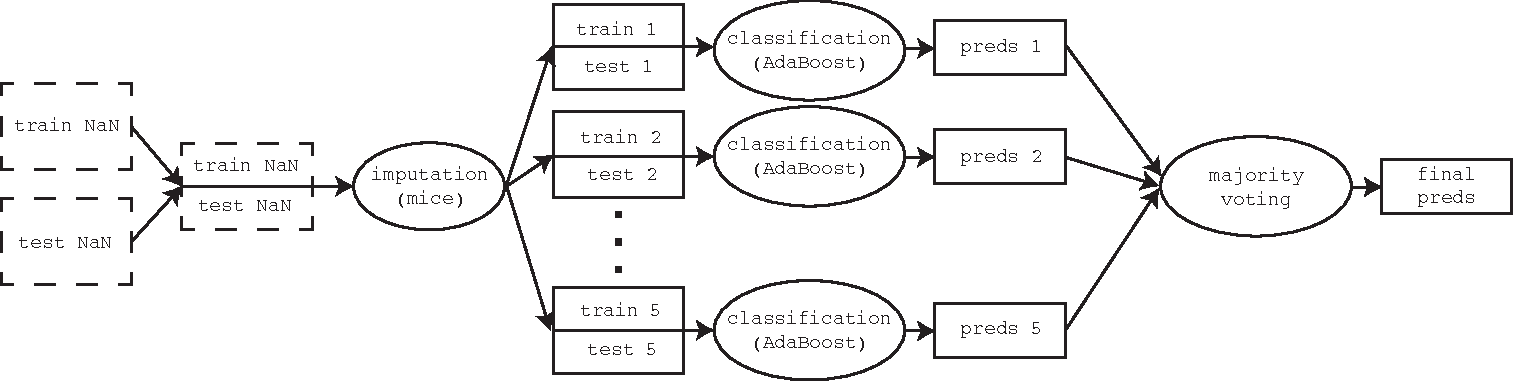
\includegraphics[width=1\columnwidth]{pipeline}
\caption{{\label{fig:pipeline} The figure illustrates the
    classification pipeline. Matrices are displayed as boxes and
    methods as ellipses; dashed lines indicate missing values.%
  }}
\end{center}
\end{figure}

\subsection{Dummy Variables}

Seven of the twelve measured variables are qualitative (workclass,
education, marital status, occupation, relationship, sex, native
country)---they are measured only at the nominal level. Since
measurements on the nominal level do not allow for a particular
ordering, a proxy method has to be used to make them suitable for
some statistical models. To this end, I defined dummy variables that take
the value 0 or 1 to indicate if a certain category is
present. Defining $n$ dummy variables for the $n$ different possible
values of a categorical feature allows for capturing the full
information in the original unmodified dataset and for using
qualitative data in a straight-forward manner.
%in regression models that are usually based on decision boundaries or linear relationships.
Transforming the dataset greatly increased its size from $D = 13$ to
$\tilde{D} = 104$ predictor variables.

\subsection{Missing Data Values}

Missing data values are a common problem in statistics due to the
failure of sensors, or the concealment of data. Thus, methods have
been put forth for the imputation of missing data points, such as case
deletion or single mean imputation~\cite{schafer2002missing}. However,
such simple methods often discard useful information and are likely to
give a rather poor result if a large part of the data is missing. The
general goal is to find unbiased estimates of the missing values. The
bias depends on the type of ``missingness'':

\begin{itemize}
\item Missing Completely At Random (MCAR)\\
  In the case of MCAR missingness, there is no dependence structure
  between the missing data and any other values. Listwise deletion
  leads to unbiased analyzes.
\item Missing At Random (MAR)\\
  In the case of MAR, the reason for missingness depends on the value
  of other non-missing predictor variables. Unbiased estimates can be
  obtained using the multiple imputation method~\cite{de2013multiple},
  which creates multiple versions of filled-in datasets.
\item Missing Not At Random (MNAR)\\
  In the case of MNAR, the reason for missingness depends on
  non-available information. Such a case might for example occur, if
  people with high income refuse to reveal their income. Imputation of
  MNAR requires explicit modeling of the reason for missingness to
  yield unbiased estimates.
\end{itemize}

For obtaining unbiased estimates with listwise deletion, the data must
be MCAR. Little's MCAR test~\cite{little1988test} is a statistical
test with the null hypothesis that the data are MCAR. I used it at the
significance level $\alpha=0.05$ to analyze the interaction structure
of the variables. The statistic was significant for the combined
dataset consisting of the training and the test set
($\chi^2 = 28018.84$, $p < 0.001$, $df=15639$). Therefore, there is
evidence that the missing values in the dataset are not MCAR; the null
hypothesis is rejected. It is not possible to distinguish between MAR
and MNAR data using observed information
only~\cite{sterne2009multiple}. Consequently, I assumed that the data
are MAR, since imputation of MNAR data would need further information
about the reason for missingness, which was not given.  Therefore,
data points were imputed using the multiple imputation method by a
technique called Multivariate Imputation by Chained Equations
(MICE)~\cite{buuren2011mice} using the \texttt{R} package
\texttt{mice} (Version~2.25). By using multiple imputations, the
algorithm incorporates the statistical uncertainty in the imputed
values. MICE is a flexible approach that can also handle continuous
and categorical variables. The general idea is to statistically model
the conditional probability of each missing variable given the
remaining variables. In detail, the MICE algorithm works as
follows~\cite{buuren2011mice,azur2011multiple}:

\begin{enumerate}
\item In the beginning, a simple imputation is carried out. To
  this end, all missing data points are replaced by random sampling
  with replacement from the observed datapoints.
\item One variable is selected at random, for example
  \emph{occupation}. An intermediate model is built, using the
  remaining variables as predictors and \emph{occupation} as target
  value. The chosen model is dependent on the target value: I used
  logistic regressions for categorical data and linear regressions for
  numerical data. The missing values in the variable \emph{occupation}
  are replaced by the predictions of the model.
\item The previous step is executed for all variables with missing
  data. For each variable, the model is trained using both the already
  imputed values and the existing values. Once all variables have been
  predicted, one cycle is complete.
\item Several cycles are performed to stabilize the imputation
  results. I used $c = 5$ cycles.
\item The entire procedure is executed multiple times to yield
  several imputed datasets. Due to the random factors, the imputed
  values will be different, while the non-missing data entries will be
  the same in all datasets. I used $m = 5$ imputations.
\end{enumerate}
The choices $c = 5$ and $m = 5$ were made due to practical
limitations, considering time limitations and avoiding overflow
errors; for the imputation
$\tilde{D} \cdot m \cdot c = 104 \cdot 5 \cdot 5 = 2600$ intermediate
models were built. A value of $m$ between 5 and 10 is a common value
for the used method~\cite{royston2011multiple} and a value of $c = 5$
is considered ``adequate''~\cite{van1999multiple}. However, recent
research shows that a higher value of $m$ might be
beneficial~\cite{white2011multiple}, which could be tested, if a more
powerful machine would be at hand.

Importantly, the MICE algorithm was used on the total dataset,
consisting of the training and the test set. This should increase the
quality of the imputed values since more training examples can be used
for building the intermediate models (Step 2 in the algorithm
outline).

In the following, the two statistical models---linear regression and
logistic regression---used for the imputations are briefly described:

\emph{Linear regression}: For the linear regression (continuous
variables), a design matrix $\mathbf{X}$ is built from the predictor
variables $x_{ij}$ ($j$th feature of the $i$th sample):
\begin{align}
\mathbf{X} = 
\begin{bmatrix}
    1 & x_{11} & x_{12} & x_{13} & \dots  & x_{1d} \\
    1 & x_{21} & x_{22} & x_{23} & \dots  & x_{2d} \\
    \vdots & \vdots & \vdots & \vdots & \ddots & \vdots \\
    1 & x_{n1} & x_{n2} & x_{n3} & \dots  & x_{nd}
\end{bmatrix}
\end{align}
The first column in the matrix enables fitting the intercept in the
regression. The solution for the weights $\hat{\beta}$---which
minimizes the squared-error loss function---is obtained using the
normal equation
$\hat{\beta} = (\mathbf{X}'\mathbf{X})^{-1}\mathbf{X}\mathbf{y}$,
where $\mathbf{y}$ is the vector consisting of the target
values. Predictions for one variable $y_i$ are made with
$\hat{y}_i = X_i\hat{\beta}$, where $X_i$ describes the features of
the $i$th sample.

\emph{Logistic regression}: Logistic regression (binary variables)
uses a logit link function to link the linear predictor $X_i\beta$ to
the probability of \emph{label 1}:
\begin{align}
  \text{Pr}(y_i = 1 | X_i) = \text{logit}^{-1}(X_i\beta) = \frac{1}{1 + e^{-X_i\beta}}
\end{align}
Logistic regression can be trained via stochastic gradient descent
(SGD). For this, the following update function is used---with a
sufficiently small learning rate $\alpha$ and
$p = \text{logit}^{-1}(X_i\beta_t)$:
\begin{align}
  \beta_{t+1} := \beta_{t} + \alpha (y-p)X_i
\end{align}
The difference $y - p$ is the error made at time step $t$ by predicting
$y$ from $X_i$ using the weight vector $\beta_{t}$.
For predicting the target value (0 or 1) of the sample $X_i$, the
hypothesis function $h(X_i)$ is used, which transforms the class
probabilities into target values:
\begin{align}
h (X_i) = 
\begin{cases}
1 & \text{if}~\text{Pr}(y_i = 1 | X_i) > 0.5\\
0 & \text{otherwise}\\
\end{cases}
\end{align}

\subsection{Pooling}
\label{sec:pooling}

I trained models and made predictions on all possible combinations of
imputed training and test sets. This results in 25 ``preliminary
hypotheses'' $\tilde{h}_{ij}$ for the $i$th sample:
$\mathbf{\tilde{h}_i} = (\tilde{h}_{i,j})_{j \in \{1, 2, \ldots, 25\}} = [\tilde{h}_{i,1}, \tilde{h}_{i,2}, \ldots, \tilde{h}_{i,25}]$. These
predictions have to be aggregated to obtain one final submission. For
the aggregation, I used the following majority voting function on the
preliminary hypotheses:
\begin{align}
\mathbf{h_i} = \text{vote}_\theta(\mathbf{\tilde{h}_i}) =
\begin{cases}
1 & \text{if}~\sum_{j = 1}^{25} h_{ij} \geq \theta\\
0 & \text{otherwise }\\
\end{cases}
\end{align}
The function predicts the class \emph{wealthy}, if at least
$\theta \in \{0, 1, 2, \ldots, 26\}$ preliminary hypotheses are
$1$. Introducing $\theta$ in the function was motivated by the local
cross-validation (next section): the default predictions of the
classifier were ``conservative''---meaning that it predominantly
predicted the class \emph{non-wealthy}---and only 54.0\,\% of actual
\emph{wealthy} samples were correctly classified. The threshold
$\theta$ serves as modulator for the ``conservatism'' of the
classifier: the higher $\theta$ is, the less likely it is that the
final prediction \emph{wealthy} will be made. The threshold
$\theta = 13$ would represent standard majority function with a
$50\,\%$ majority.  Figure~\ref{fig:tuning} shows the trade-off
between specificity and sensitivity for increasing values of
$\theta$. It can be seen that the accuracy is not greatly affected by
the threshold $\theta$: a higher sensitivity is directly traded-off
with a smaller specificity. The maximum accuracy was achieved at
$\theta = 9$.

\begin{figure}[h]
  \centering
  \includegraphics[width=0.5\textwidth]{../Python/theta}
  \caption{Accuracy, sensitivity, and specificity in dependence of the
    threshold $\theta$. The accuracy stays roughly the same for
    $6 \leq \theta \leq 25$. In contrast, the sensitivity falls and
    the specificity rises for increasing values of $\theta$.}
  \label{fig:tuning}
\end{figure}


\subsection{Cross-Validation}
\label{sec:cross}

To evaluate submissions and determine the ranks of participants, the
Kaggle challenge used the 0--1 loss. While the score on the public
leaderboard is the best validation of the methods employed, only one
submission could be submitted per participant and day. To evaluate my
approach more frequently, I implemented a local ($k = 5$)-fold
cross-validation. In each fold, a model was trained on $\frac{4}{5}$
of the data and tested on the remaining samples from all five imputed
datasets. Therefore, $k \cdot m \cdot m = 5 \cdot 5 \cdot 5 = 125$
accuracy values were obtained from which the mean was calculated to
get a final cross-validation accuracy for each model. The
cross-validation achieved similar results to the public Kaggle
evaluation (Table~\ref{tab:localpublic}).

\begin{table}[h]
  \centering
  \begin{tabular}{lll}
    \toprule
    Method & Local Score (\%) & Global Score (\%)\\
    \midrule
    AdaBoost with 1 imputation & 83.886 & 84.205\\
    Random Forest with 5 imputations & 82.726 & 85.056\\
    SVM with 5 imputations & 84.413 & 85.494\\
    AdaBoost with 5 imputations & & \\
    SVM with 25 imputations &  & 85.718\\
    \bottomrule
  \end{tabular}
  \caption{{Comparing local and public scores}}
  \label{tab:localpublic}
\end{table}

Each fold in the cross-validation contained 2100 test samples and 8400
training samples. Since the classes \emph{wealthy} and
\emph{non-wealthy} are not equally distributed, a confusion matrix can
give a more detailed picture of the classifier performance. After
predicting the labels for all five folds, the following confusion
matrix was obtained:

\begin{table}[h]
\centering
\begin{tabular}{l|l|c|c|c}
\multicolumn{2}{c}{}&\multicolumn{2}{c}{Predicted class}&\\
\cline{3-4}
\multicolumn{2}{c|}{}&wealthy & non-wealthy &\multicolumn{1}{c}{Total}\\
\cline{2-4}
\multirow{2}{*}{Actual class}& wealthy & $TP = 1351$ & $FN = 1149$ & $TP+FN = 2500$\\
\cline{2-4}
& non-wealthy & $FP = 546$ & $TN = 7454$ & $FP+TN = 8000$\\
\cline{2-4}
\multicolumn{1}{c}{} & \multicolumn{1}{c}{Total} & \multicolumn{1}{c}{$TP+FP=1897$} & \multicolumn{1}{c}{$FN+TN = 8603$} & \multicolumn{1}{c}{$N = 10500$}\\
\end{tabular}
\end{table}
From the confusion matrix, sensitivity and specificity can be calculated:
\begin{align}
\text{Sensitivity} &= \frac{TP}{TP + FN} = 54.0\,\%\\
\text{Specificity}    &= \frac{TN}{TN + FP} = 93.2\,\%\\
\end{align}
These statistics show that almost all non-wealthy samples are
correctly classified, while only slightly more than half of the
wealthy samples are correctly classified. The confusion matrix implies
that the classifier is ``conservative'': it avoids classifying samples
as \emph{wealthy}. The high overall accuracy is mainly caused by
correctly classifying non-wealthy samples.

\subsection{The Classifier}

Section~\ref{sec:cross} shows the different classifiers that were
compared. The best performing classifier was a support vector machine
(SVM). For running the algorithm \texttt{Python~2.7.11} was used with
the package \texttt{scikit-learn} in Version~0.17.0.

The choice of an SVM was motivated by the following points:

\begin{enumerate}
\item SVMs work ``out-of-the-box'' on many different problems~\cite{russell2003artificial}.
\item SVMS work in high-dimensional spaces ($\tilde{D} = 104$)
\item SVMs aim to minimize the generalization error by finding a
  decision boundary that maximizes the margin.
\item SVMs allow for \emph{transductive learning} using transductive
  SVMs. Therefore, the information in the unlabeled test data can be
  incorporated in the training process, possibly improving the
  accuracy.
\item SVMs showed the best performance in the local cross-validation.
%\item Using the \emph{kernel trick}, data can be embedded in a
%  higher-dimensional space, which might make the dataset easily
%  separable.
\end{enumerate}

If $D$ is the number of features, SVMs build a ($D-1$)-dimensional
hyperplane that tries to maximize the margin between the two
classes. The support vectors are the samples on the margin for the
positive class and the negative class. The maximum-margin hyperplane
is the hyperplane ``right in the middle'' of the support vectors.

The classifier is of the form $f(\mathbf{x}) = w^T\mathbf{x} + b$ and
the corresponding classification function is
$h(\mathbf{x}) = sign(w^T\mathbf{x} + b)$, with $\mathbf{x}$ being the
feature vector, $w$ the coefficient vector and $b$ the intercept
term. The target variables $y_i$ for SVMs are $-1$ (\emph{non-wealthy})
and $1$ (\emph{wealthy}), instead of $0$ and $1$. To train the
classifier, the goal is to find $w, b$ such that the resulting
decision boundary maximizes the margin.
%A soft-margin is used with the hinge-loss function:
%\begin{align}
%  \max\left(0, 1 - y_i(\vec{w}\cdot \vec{x_i} + b)\right)
%\end{align}.
Therefore, the following optimization problem---known as the
\emph{primal representation}--- is solved:
\begin{align}
  & \min ||\mathbf{w}||^2 + C \sum_{i = 1}^N\zeta_i\\
  & \text{subject to the constraints:}\\
 & \mathbf{w}^T\mathbf{x}_i \geq + 1-\zeta_i, \text{for}~y_i =
  +1\\
 & \mathbf{w}^T\mathbf{x}_i <-1+\zeta_i, \text{for}~y_i =
  -1\\
& \zeta_i \geq 0, \forall i
\end{align}
To allow for non-linearly separable datasets and make the SVM less
sensitive to outliers, the variables $\zeta_i$ allow for introducing
``slackness'' into the constraints, such that not every sample has to
lie at the correct side of the margin. If $0 < \zeta_i \leq 1$, the
sample is between the margin and the correct side of hyperplane; if
$\zeta > 1$, the sample is misclassified. The hyperparameter $C$
allows for trading off structural error and training error: a value
close to 0 specifies that violating the margin constraint---that each
sample is at the correct side of the margin---is of not much
consequence; greater values put more emphasis on satisfying the margin
constraint for each data point.


To find $w$ and $b$, it is often more convenient to use the \emph{dual
  representation}, which can be derived from the primal
form~\cite{russell2003artificial}:
\begin{align}
\label{eq:dual}
\text{arg}\max_\alpha\sum_j\alpha_j - \frac{1}{2}\sum_{j,k}\alpha_j\alpha_ky_jy_k(\mathbf{x_j} \cdot \mathbf{x_k})
\end{align} subject to the constraints: $\alpha_j \geq 0$ and
$\sum_j\alpha_jy_j=0$. The variable $y_i \in \{-1, 1\}$ represents the
class of $x_i$ and $\alpha$ is the weights vector that assigns a weight
$\alpha_j$ to each data point. The \emph{support vectors} are the
samples for which the weights $a_j$ are non-zero. 
This optimization problem can be solved using
quadratic programming, for which several libraries
exist. I used the solution provided by the \texttt{libsvm}
library~\cite{libsvm2011}.

To extend SVMs to non-linear classification, the \emph{kernel trick}
can be used, with which data can be embedded in a higher-dimensional
space. The kernel $K(\mathbf{x_j}, \mathbf{x_k})$ is then applied to
the dot products of feature vectors in
Equation~\ref{eq:dual}. Therefore, the equation becomes:
\begin{align}
\label{eq:dualkernel}
  \text{arg}\max_\alpha\sum_j\alpha_j - \frac{1}{2}\sum_{j,k}\alpha_j\alpha_ky_jy_kK(\mathbf{x_j}, \mathbf{x_k})
\end{align} 
Practically, this means that the problem of finding a linear separator
is shifted to a higher dimensional feature space. Mapping back this
linear separator to the original feature space results in a non-linear
decision boundary.  For the given problem, a Gaussian radial basis
function kernel was used:
\begin{align}
K(\mathbf{x_j}, \mathbf{x_k}) = \exp(-\gamma||\mathbf{x_j} - \mathbf{x_k} ||^2)
\end{align}
The two hyperparameters of the SVM, $C$ and
$\gamma$,  were chosen using grid-search in the cross-validation.


Before training, each variable in the combined dataset, consisting of
training and test set, was scaled to zero mean and unit variance using
the following formula:
\begin{align}
  x' = \frac{x - \bar{x}}{\sigma}
\end{align}
In the formula, $x$ is the original value, $x'$ the new value, and
$\bar{x}$ and $\sigma$ mean and standard deviation of the
variable. Scaling ensures that features with a greater range do not
dominate features with smaller ranges~\cite{hsu2003practical}.

\subsection{Transductive Learning}

Since the test data is known at training time, this information can be
used for using semi-supervised methods than can better capture the
underlying distribution. I made use of the self-learning method: at
first, the unlabeled data was labeled by predicting their labels using
a SVM trained on the provided training set. Afterward, another SVM was
trained using the combined dataset consisting of training and the test
set and the final predictions for the test set were made. The approach
did not improve the classification performance.

Two more sophisticated approaches---using the implementations of
\texttt{semisup-learn}\footnote{\url{https://github.com/tmadl/semisup-learn}}---
Contrastive Pessimistic Likelihood Estimation
(CPLE)~\cite{loog2016contrastive} and Transductive
SVMs~\cite{bennett1999semi,gieseke2014fast} were terminated
prematurely since training was not finished after 24 hours.

\section{Results \& Discussion}
\label{sec:results}

In total, I made 10 submissions during the competition. The best
submission resulted in an accuracy of $85.718\,\%$, which corresponds
to the $3^{\text{rd}}$ position out of 26 participants when
finishing this report.

In summary, the main challenge lay in imputing the missing data
values. Afterward, standard classification techniques could be
used. The threshold parameter $\theta$ of the majority voting had no
substantial influence on the classification performance. Also,
different classifiers did not greatly affect the achieved accuracy:
support vector machines, random forest classification, and AdaBoost
classifiers yielded similar results, as shown in
Table~\ref{tab:localpublic}.

The use of self-supervised learning did not have a positive effect on
the classification performance; this is in line with findings other
studies, showing that semi-supervised methods do not necessarily lead
to improved performances and can even lead to a lower
accuracy~\cite{zhu2005semi}. It might be that semi-supervised methods
would have had a greater effect, if the number of training samples
would have been substantially smaller. 

Since the ground truth labels of the test set were not revealed, error
statistics could only be computed based on the 0--1 loss on the public
leaderboard and on the local cross-validation. The restriction of one
submission per day increased the difficulty of the validation. My
public score of $85.718\,\%$---which is $0.00876$ below the best
performing score in the competition ($86.594\,\%$) and $0.00232$ below
the best performing method of the Delve
project~\footnote{\url{http://www.cs.toronto.edu/~delve/data/adult/adultDetail.html}}---is
an indicator that little improvement will be possible beyond my
approach. Compared to the UCI dataset, the given dataset had a smaller
amount of labeled data and more missing values, which made the Kaggle
classification task more challenging. Using standard state-of-the-art
classifiers, the maximum possible performance of the given dataset
will be possibly capped below 100\,\% due to mistakes during data
acquisition, such as deliberate misinformation or transcription
errors. Moreover, the used variables might only have limited
explanatory power: additional variables, such as political view,
morale, or number of children may be needed to increase the
explainable variation.

Due to the concealment of categorical variables, I did not consider
manual feature engineering such as grouping certain levels of the
categorical (dummy) variables.

Many steps in the classification pipeline were time-consuming, taking
several hours to complete. In the future, more processing power could
help to increase the classification performance. For example, using a
larger amount of imputed datasets could capture the uncertainty in the
imputed values to a greater degree and another method for
transductive learning could help to increase the classification performance.
% The number of base classifiers---the decision stumps---in the
% AdaBoost classifier could be further increased.
%Moreover, the CPLE framework could be
%tested with classifiers that showed good performance in the
%cross-validation without transductive learning, such as random forests
%or support vector machines.

My code for this competition can be found at:\\
\url{https://github.com/Pold87/ml-final-ass}

\emph{Word Count}: 3403
\printbibliography
\end{document}


%  LocalWords:  missingness transductive
